% !TEX TS-program = xelatex
% !TEX encoding = UTF-8 Unicode
\documentclass[11pt,a4paper]{article}
\usepackage{amsmath,amssymb}
\usepackage{empheq}
\usepackage[semibold]{ebgaramond}
\usepackage[cmintegrals,cmbraces]{newtxmath}
\usepackage{ebgaramond-maths}
\usepackage{bm}
\usepackage[OMLmathrm, OMLmathsfit, rmdefault=mdugm]{isomath}
\usepackage{tocbibind}
\usepackage{graphicx}
\graphicspath{{./pics/}}
\usepackage{wrapfig}

\makeatletter
  \DeclareSymbolFont{ntxletters}{OML}{ntxmi}{m}{it}
  \SetSymbolFont{ntxletters}{bold}{OML}{ntxmi}{b}{it}
  \re@DeclareMathSymbol{\leftharpoonup}{\mathrel}{ntxletters}{"28}
  \re@DeclareMathSymbol{\leftharpoondown}{\mathrel}{ntxletters}{"29}
  \re@DeclareMathSymbol{\rightharpoonup}{\mathrel}{ntxletters}{"2A}
  \re@DeclareMathSymbol{\rightharpoondown}{\mathrel}{ntxletters}{"2B}
  \re@DeclareMathSymbol{\triangleleft}{\mathbin}{ntxletters}{"2F}
  \re@DeclareMathSymbol{\triangleright}{\mathbin}{ntxletters}{"2E}
  \re@DeclareMathSymbol{\partial}{\mathord}{ntxletters}{"40}
  \re@DeclareMathSymbol{\flat}{\mathord}{ntxletters}{"5B}
  \re@DeclareMathSymbol{\natural}{\mathord}{ntxletters}{"5C}
  \re@DeclareMathSymbol{\star}{\mathbin}{ntxletters}{"3F}
  \re@DeclareMathSymbol{\smile}{\mathrel}{ntxletters}{"5E}
  \re@DeclareMathSymbol{\frown}{\mathrel}{ntxletters}{"5F}
  \re@DeclareMathSymbol{\sharp}{\mathord}{ntxletters}{"5D}
  \re@DeclareMathAccent{\vec}{\mathord}{ntxletters}{"7E}
\makeatother

\usepackage{array}
\usepackage{enumitem}
% to produce a comma between multiple footnotes / https://tex.stackexchange.com/questions/40072/incompatibility-between-footmisc-option-multiple-and-hyperref/62091#62091
\let\oldFootnote\footnote
\newcommand\nextToken\relax
\renewcommand\footnote[1]{%
    \oldFootnote{#1}\futurelet\nextToken\isFootnote}
\newcommand\isFootnote{%
    \ifx\footnote\nextToken\textsuperscript{,}\fi}

\defaultfontfeatures{Ligatures=TeX} % makes this a feature for all selected fonts
\usepackage{esint}
\usepackage{polyglossia}
\setmainlanguage{english}
\usepackage[text={18cm,26cm},centering]{geometry} % 
\usepackage{natbib}
\usepackage{mdframed}
\usepackage{lipsum}
\usepackage[usenames,dvipsnames,svgnames,table]{xcolor}
\usepackage{hyperref}
\usepackage{url}
\usepackage[export]{adjustbox}

\hypersetup{
  colorlinks,
  citecolor=bleuSU,
  linkcolor=bleuSU
}
\definecolor{bleuSU}{RGB}{26,39,101}

\usepackage[normalem]{ulem}
\makeatletter
\renewcommand*{\uuline}{%
  \bgroup
  \UL@setULdepth
  \markoverwith{%
    \lower\ULdepth\hbox{%
      \kern-.03em%
      \vtop{%
        \hrule width.2em%
        \kern 0.6pt % distance between the two underlines
        \hrule
      }%
      \kern-.03em%
    }%
  }%
  \ULon
}
\makeatother
\setlength{\ULdepth}{-2pt}  % distance from double underline to letter

\usepackage{environ}
\newtoggle{corrige}

\NewEnviron{answer}{%
  \iftoggle{corrige}
    {\begin{mdframed}\textbf{Answer: } \BODY\end{mdframed}}
    {}%
  }

\newcommand{\delS}{\delta S}
\newcommand{\delA}{\delta A}
\newcommand{\delh}{\delta h}
\newcommand{\delt}{\delta t}
\newcommand{\delz}{\delta z}
\newcommand{\delbx}{\delta \matrixsym x}
\newcommand{\lp}{\left(}
\newcommand{\rp}{\right)}
\newcommand{\itA}{\textit A}
\newcommand{\itB}{\textit B}
\newcommand{\dAB}{\mathcal D_{AB}}
\newcommand{\bA}{\matrixsym A}
\newcommand{\bff}{\matrixsym{f}}
\newcommand{\bF}{\matrixsym{F}}
\newcommand{\bj}{\matrixsym{j}}
\newcommand{\bJ}{\matrixsym J}
\newcommand{\bn}{\matrixsym{n}}
\newcommand{\bN}{\matrixsym N}
\newcommand{\bP}{\matrixsym{P}}
\newcommand{\br}{\matrixsym r}
\newcommand{\bt}{\matrixsym t}
\newcommand{\be}{\matrixsym e}
\newcommand{\bu}{\matrixsym u}
\newcommand{\bv}{\matrixsym v}
\newcommand{\bw}{\matrixsym w}
\newcommand{\bx}{\matrixsym x}
\newcommand{\pd}[2]{\frac{\partial #1}{\partial #2}}
\newcommand{\D}[2]{\frac{D #1}{D #2}}
\newcommand{\dd}[2]{\frac{\mathrm d #1}{\mathrm d #2}}
\newcommand{\dA}{\mathrm dA}
\newcommand{\dV}{\mathrm dV}
\newcommand{\dS}{\mathrm dS}
\newcommand{\prg}[1]{\paragraph{$\rhd$ #1}}
\newcommand{\alphaijkl}{\alpha_{ijkl}}
\newcommand{\Aijkl}{A_{ijkl}}
\newcommand{\delij}{\delta_{ij}}
\newcommand{\sigij}{\sigma_{ij}}
\newcommand{\sigji}{\sigma_{ji}}
\newcommand{\sigxy}{\sigma_{xy}}
\newcommand{\matL}{\mathcal L}
\newcommand{\matO}{\mathcal O}
\newcommand{\matS}{\mathcal S}
\newcommand{\kij}{k_{ij}}
\newcommand{\tensor}[1]{\smash{\uuline{#1}{}}}
\setlength{\parindent}{0pt} % remove indent

\setlist[enumerate]{topsep=0pt,itemsep=-1ex,partopsep=1ex,parsep=1ex}

\begin{document}
\setlength{\unitlength}{1cm}
\noindent
\parbox{\textwidth}{
\textsc{
Sorbonne Université  
\hfill
Year 2021-2022
}
}
\parbox{\textwidth}{
\textsc{
Faculté des Sciences
\hfill
Physics of Fluids \& Nonlinear Physics
}
}

\begin{center}
\Large
\textbf{Hydrodynamics} \\ 
\textsl{Tutorial 5: Saint-Venant equations} \\[1ex]
\end{center}

\section{Dam break}
\togglefalse{corrige}

%\begin{figure}[ht]
%    \centering
%    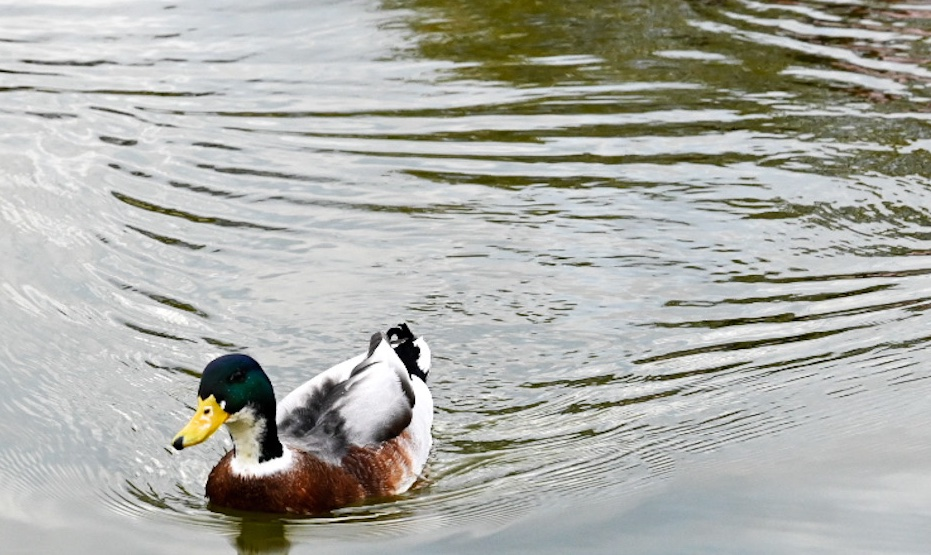
\includegraphics[width=7cm]{duck_wave_pattern.jpg}
%    \caption{\textbf{Duck waves.} A duck moving around in a pond produces a wave pattern in its wake (Jardin des Tuileries, Paris. Photograph AA).}
%    \label{fig:wave_pattern}
%\end{figure}
We set out to describe the dynamics resulting from the rupture of a dam. The liquid contained is supposed to have a initial depth noted $h_0$ and no velocity, and occupies $x<0$. The dam is located at $x=0$ and breaks at $t=0$. In the problem we model the evolution of the liquid with the Saint-Venant equations.

The Saint-Venant equations describing the motion of a thin inertial liquid film read:
\begin{subequations}
\label{eq:curvature_radius}
\begin{empheq}[left=\empheqlbrace]{alignat=2}
h_t + (hu)_x &=& 0\\
u_t + uu_x+gh_x &=& 0
\end{empheq}
\end{subequations}
\begin{enumerate}
\item We start by considering a still liquid (depth $h_0$ and no velocity). By linearising the Saint-Venant equations around this base flow, show that they admit plane wave solutions propagating at $\pm c$. Give the value of the celerity $c$. Does it depend on the wavelength?
\item Show that the (full) Saint-Venant equations can be rewritten as:
\begin{equation}
\left(\frac{\partial}{\partial t} + \left(u \pm c\right)\frac{\partial}{\partial x}\right)\left(u\pm 2c\right)=0,
\end{equation}
\item Deduce that some quantities (called the \textit{Riemann invariants}) are preserved along the curves $\frac{\mathrm dx}{\mathrm dt} = u\pm c$ (called \textit{characteristics}) noted respectively $C^+$ and $C^-$ in the following.
\item Represent the characteristics for the region far from the dam, where the water is undisturbed. Supposing that the set of characteristics cross each other, deduce the value of $h$ and $u$ there, and the real shape of the characteristics.
\item Show that this region is bounded by $x < -c_0 t$.
\item Supposing that the $C^+$ characteristics enter into the domain  $x > -c_0 t$, show that $u$ and $h$ are constants along the $C^-$ curves, and that these are lines.
\item At $t=0$ the fluid only occupies the region $x<0$ so the $C^-$ characteristics must all come from zero and satisfy
\begin{equation}
\frac{x}{t} = u - c
\end{equation}
but also $u+2c = 2c_0$.
\item Deduce that the shape and velocity of the water satisfy at all instants:
\begin{subequations}
\label{eq:height_velocity}
\begin{empheq}[left=\empheqlbrace]{alignat=2}
h(x,t) &=& \frac{h_0}{9}\left(2-\frac{x}{c_0t}\right)^2\\
u(x,t) &=& \frac{2}{3}\left(c_0+\frac{x}{t}\right)
\end{empheq}
\end{subequations}
\item Compute the real shape of the characteristics and conclude on the validity of the assumptions.
\end{enumerate}
\bibliographystyle{jfm}
\bibliography{biblio_tuto}
\end{document}